\documentclass[9pt]{beamer}

\usepackage[T1]{fontenc}
\usepackage{color}
\usepackage{graphicx}
\usepackage{natbib}
\usepackage{tikz}
\usepackage{pgfgantt}

\usetheme{Boadilla}

\definecolor{rd}{HTML}{2F2A40}
\definecolor{methods}{HTML}{C6C6C6}
\definecolor{research}{HTML}{8F84BE}
\definecolor{skills}{HTML}{7A7A7A}
\definecolor{rc}{HTML}{AC152A} 

\usefonttheme{professionalfonts}

\title[Climate Topography]{A Topography of Climate Change Research}
\subtitle{}
\author{Max Callaghan}
\institute[MCC]{
	
\includegraphics[height=1cm,width=2cm]{MCC_Logo_RZ_rgb.jpg}
%	\,
%	
\includegraphics[height=1cm]{hertie_logo.png}
}

\newtheorem*{remark}{}

\bibliographystyle{apalike}

\begin{document}
	
\begin{frame}
	\titlepage
\end{frame}

\addtobeamertemplate{frametitle}{}{%
	\begin{tikzpicture}[remember picture,overlay]
	\node[anchor=north east,yshift=2pt] at (current page.north east) {
\includegraphics[height=0.8cm]{MCC_Logo_RZ_rgb.jpg}};
	\end{tikzpicture}}

\begin{frame}{Context}

\begin{columns}
	\begin{column}{0.5\linewidth}
		\begin{center}
		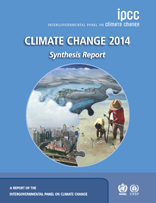
\includegraphics[width=0.6\linewidth]{syrcover.png}
		\end{center}
	\end{column}
	\begin{column}{0.5\linewidth}
	\begin{center}
		\begin{itemize}
			\item To contribute evidence-based policy-making on climate change, the IPCC aims to \textit{comprehensively} assess  
			\item These assessments should be aim to balance legitimacy, credibility and relevance \citep{Cash2001}
		\end{itemize}
	\end{center}
	\end{column}
	\end{columns}

\end{frame}

\begin{frame}{Motivation}

\begin{columns}
	\begin{column}{0.5\linewidth}
		\begin{center}
%			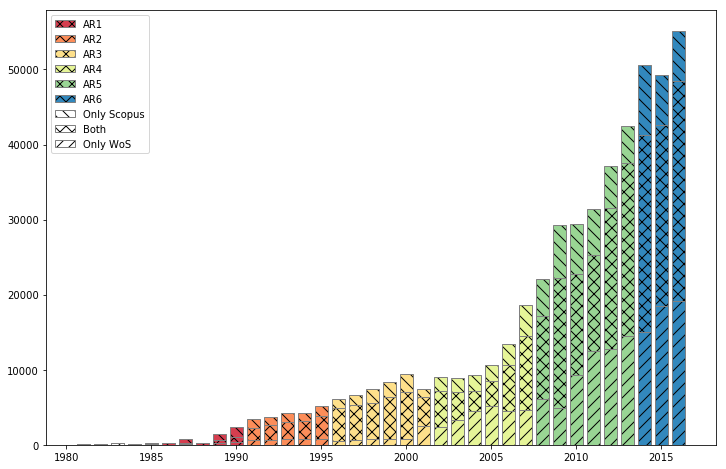
\includegraphics[width=0.85\linewidth]{../plots/wos_scopus_docs_time.png}
\begin{figure}
	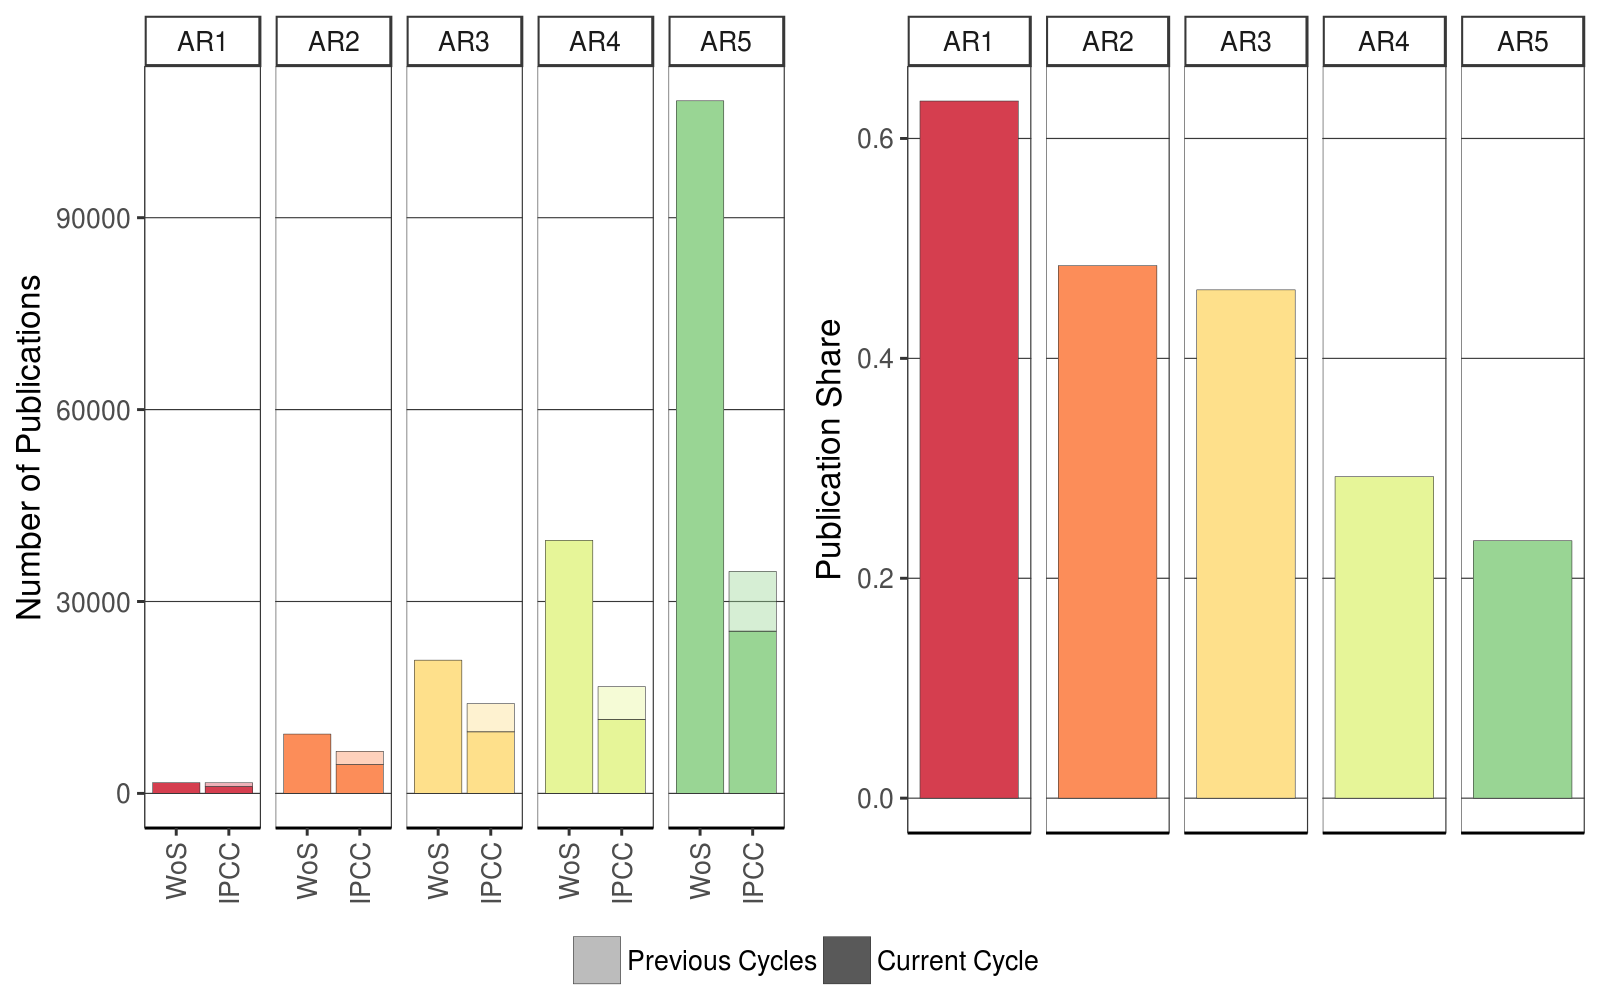
\includegraphics[width=0.85\linewidth]{merged_IPCC_spectral.png}
	\caption{Source: \citet{Minx2017l} }
\end{figure}
		\end{center}
	\end{column}
	\begin{column}{0.5\linewidth}
		\begin{center}
			\begin{itemize}
				\item Comprehensive, credible and relevant assessments become
				more challenging as the literature grows
			\end{itemize}
		\begin{remark}[]
			To understand, and to aid, scientific assessments of climate change, we need to machine read the literature
		\end{remark}
		\end{center}
	\end{column}
\end{columns}

\end{frame}

\begin{frame}{Approach - Words, words, words}

\begin{columns}
	\begin{column}{0.5\linewidth}
		\begin{center}
			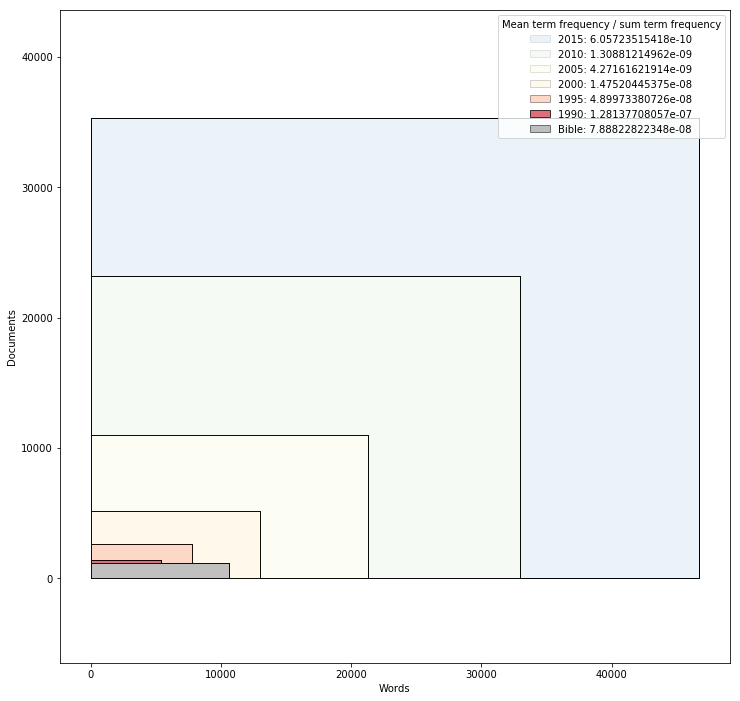
\includegraphics[width=\linewidth]{volume_variety_bible.png}
		\end{center}
	\end{column}
	\begin{column}{0.5\linewidth}
		\begin{center}
			\begin{itemize}
				\item Topic modelling is a way of reducing the dimensionality of a corpus of documents
				\item A large matrix of documents x words is factorised by
				a matrix of topics x words and a matrix of topics x documents
			\citep{Lee1999}
				\item Topics describe the latent structure of the document corpus
				
			\end{itemize}
		\end{center}
	\end{column}
\end{columns}

\end{frame}

\begin{frame}{Preliminary results - explanation}

\begin{columns}
	\begin{column}{0.5\linewidth}
		\begin{center}
			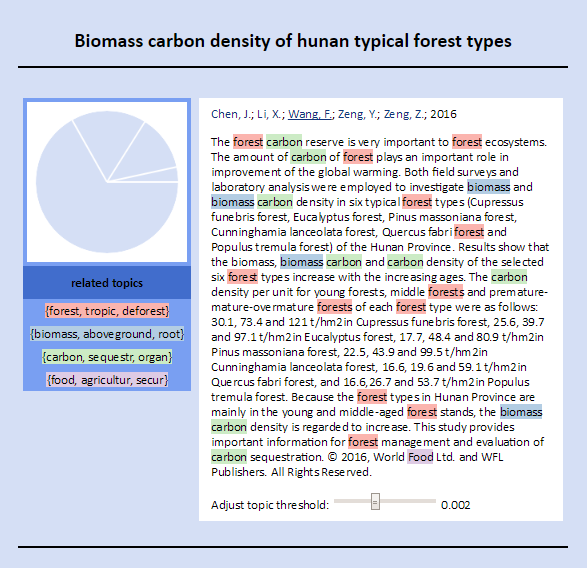
\includegraphics[width=\linewidth]{../plots/biomass_eg.png}
		\end{center}
	\end{column}
	\begin{column}{0.5\linewidth}
		\begin{center}
			\begin{itemize}
				\item Documents are mixtures of topics, based on the words which occur in them
			\end{itemize}
		\end{center}
	\end{column}
\end{columns}

\end{frame}


\begin{frame}{Preliminary results - structure}

\begin{columns}
	\begin{column}{0.6\linewidth}
		\begin{center}
			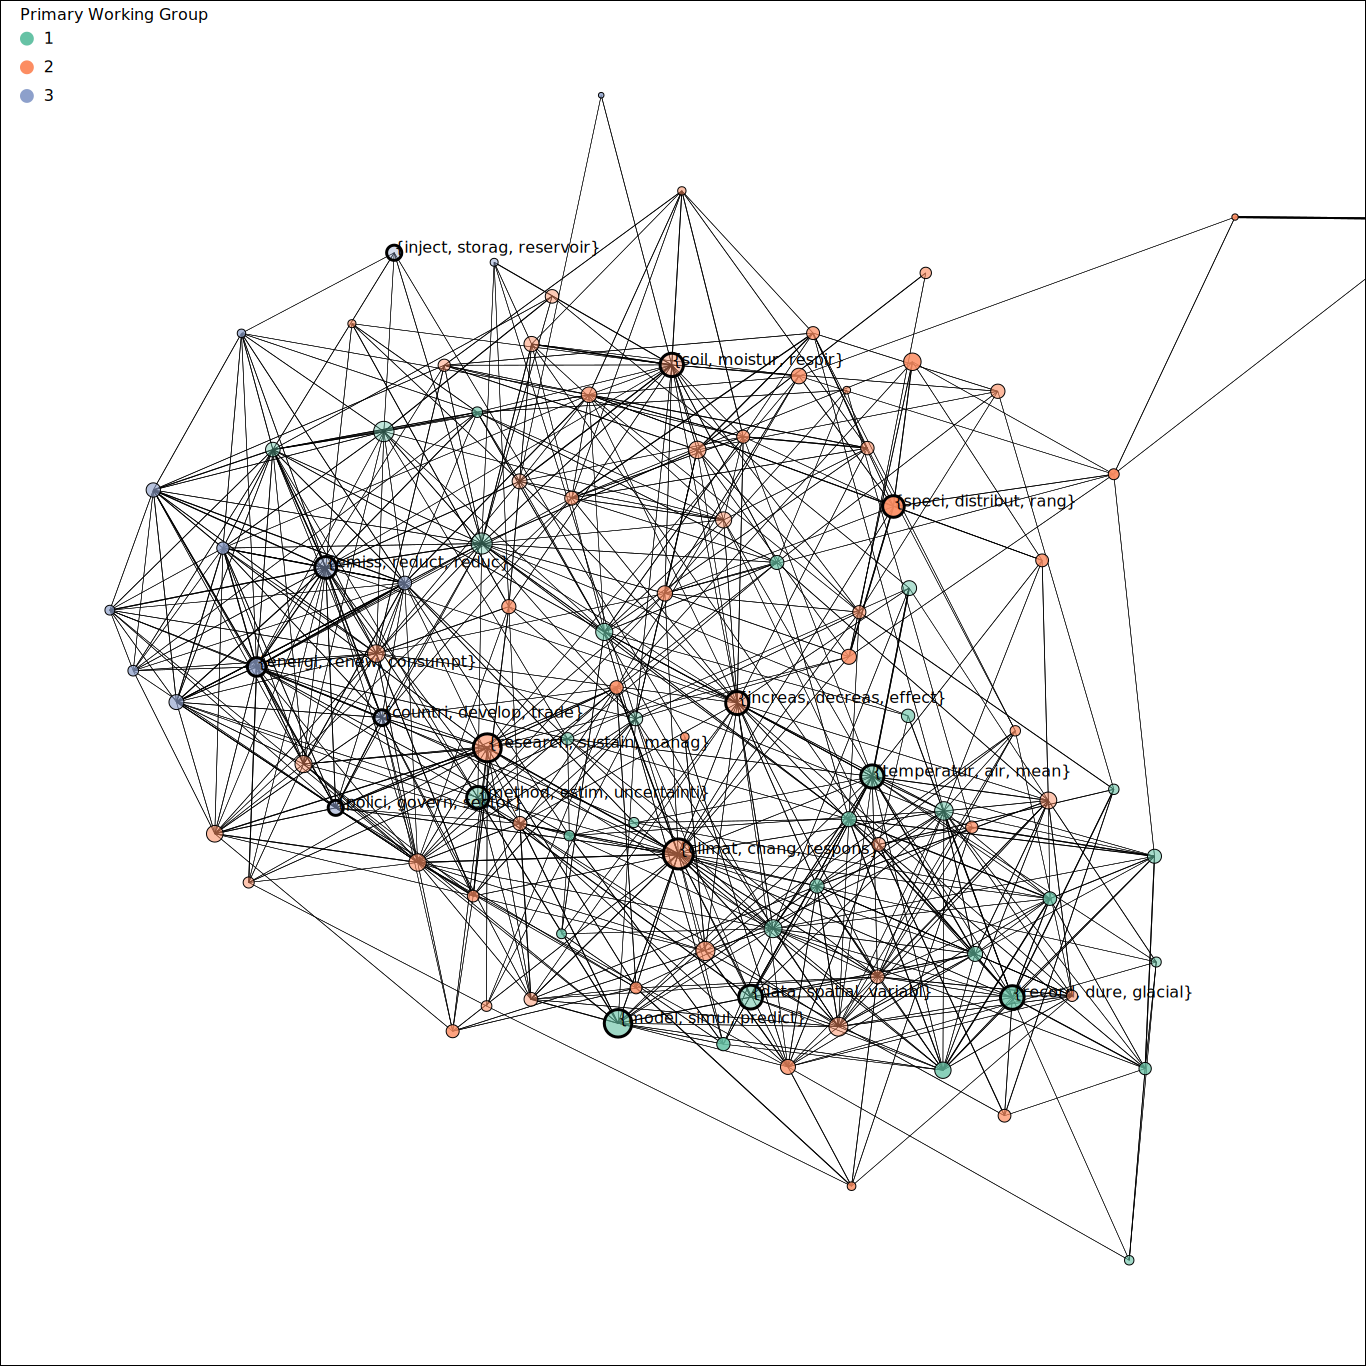
\includegraphics[width=0.85\linewidth]{../plots/network_wg_372.PNG}
		\end{center}
	\end{column}
	\begin{column}{0.4\linewidth}
		\begin{center}
			\begin{itemize}
				\item A network of comprehensible topics is generated with 100 topics
				\item Topics can be matched to the IPCC working group from which the majority of the topic documents are referenced in
				\item Topics from the same working group are \textbf{significantly} more likely to be correlated with each other than those which are not
			\end{itemize}
		\end{center}
	\end{column}
\end{columns}

\end{frame}

\begin{frame}{Preliminary results - structure}

\begin{columns}
	\begin{column}{0.6\linewidth}
		\begin{center}
			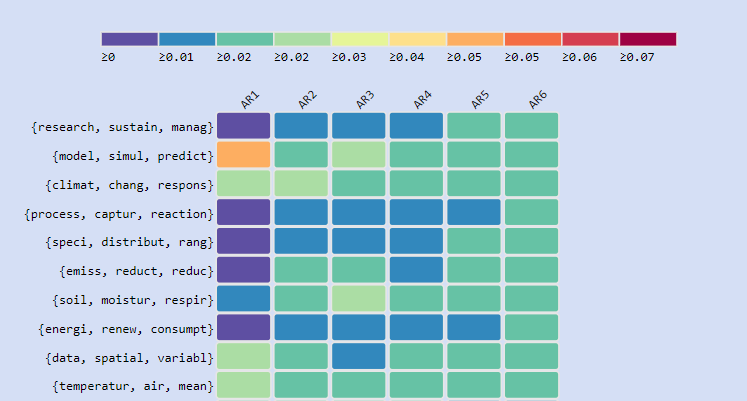
\includegraphics[width=0.85\linewidth]{../plots/shares_10_372.PNG}
			
			\medskip
			
			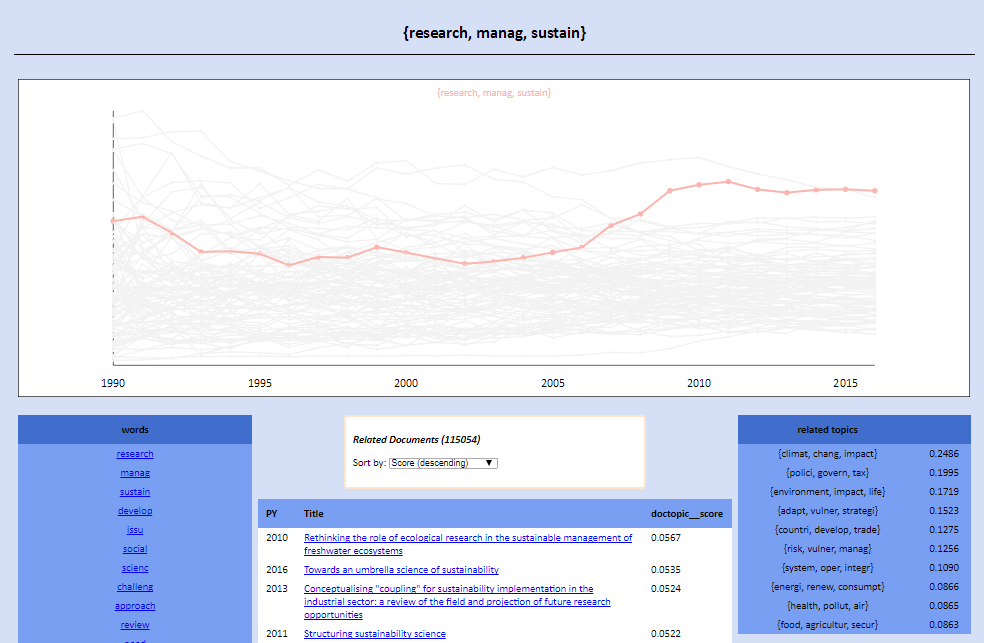
\includegraphics[width=0.85\linewidth]{../plots/sustainability.PNG}
		\end{center}
	\end{column}
	\begin{column}{0.4\linewidth}
		\begin{center}
			\begin{itemize}
				\item In later assessment periods, the largest topic is on research priorities and sustainability
			\end{itemize}
		\end{center}
	\end{column}
\end{columns}

\end{frame}

\begin{frame}{Preliminary results - growth}

\begin{columns}
	\begin{column}{0.6\linewidth}
		\begin{center}
			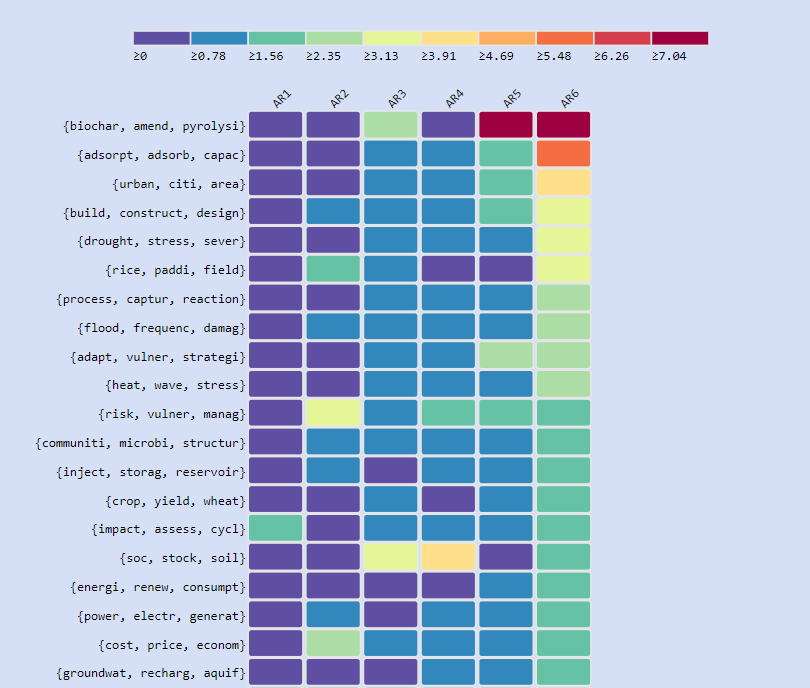
\includegraphics[width=\linewidth]{../plots/top_20_372.png}
		\end{center}
	\end{column}
	\begin{column}{0.4\linewidth}
		\begin{center}
			\begin{itemize}
				\item Negative emissions related topics have shown strong growth since the end of AR5
				\item As have topics on cities and extreme weather events
			\end{itemize}
		\end{center}
	\end{column}
\end{columns}

\end{frame}

\begin{frame}{Preliminary results - gaps in coverage}

\begin{columns}
	\begin{column}{0.6\linewidth}
		\begin{center}
			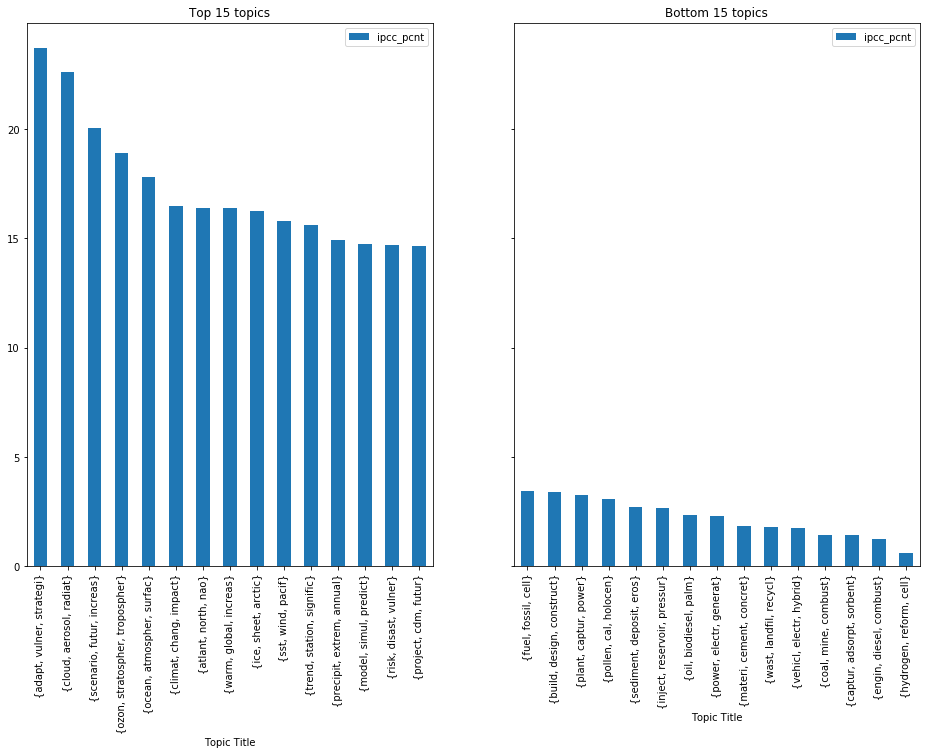
\includegraphics[width=\linewidth]{../plots/ipcc_topics_65.png}
		\end{center}
	\end{column}
	\begin{column}{0.4\linewidth}
		\begin{center}
			\begin{itemize}
				\item The physical science aspects of climate change, as well topics on impacts, adaptation and scenarios are well covered by the IPCC
				\item ``Niche'' topics on specific technological solutions, are less well covered
			\end{itemize}
		\end{center}
	\end{column}
\end{columns}

\end{frame}

\begin{frame}{Next steps}

\begin{columns}
%	\begin{column}{0.6\linewidth}
%		\begin{center}
%			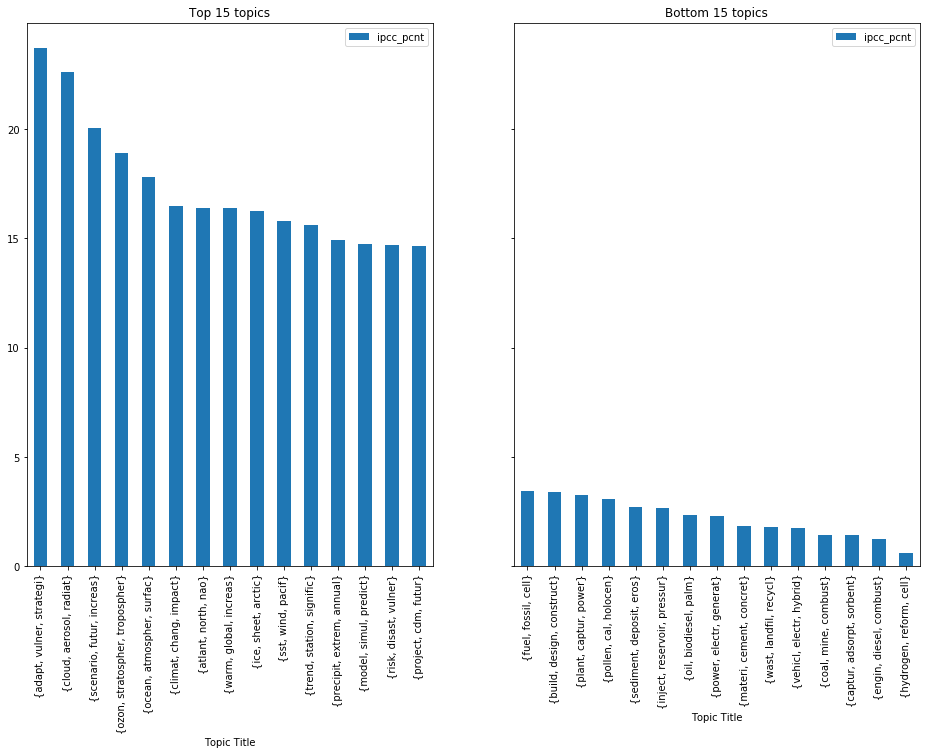
\includegraphics[width=\linewidth]{../plots/ipcc_topics_65.png}
%		\end{center}
%	\end{column}
	\begin{column}{0.7\linewidth}
		\begin{center}
			\begin{itemize}
				\item Can I get a clearer research question, and make the analysis less descriptive?
			\end{itemize}
		\end{center}
	\end{column}
\end{columns}

\end{frame}


%\begin{frame}{Outlook}
%
%\begin{figure}
%
%\tiny
%
%\begin{ganttchart}[
%	y unit title=0.3cm,
%	y unit chart=0.5cm,
%	x unit= 0.2cm,
%	vgrid,hgrid,
%	vgrid={{dotted,dotted,black}},
%	title height=1,
%	%     title/.style={fill=none},
%	title label font=\bfseries\scriptsize,
%	%bar/.style={fill=blue},
%	bar height=0.7,
%	bar label font=\tiny,
%	%   progress label text={},
%	group right shift=0,
%	group top shift=0.7,
%	group height=.3,
%	group peaks width={0.2},
%	inline]{1}{42}
%	\gantttitle{2017}{9}
%	\gantttitle{2018}{12}
%	\gantttitle{2019}{12}
%	\gantttitle{2020}{9} \\
%	\gantttitlelist{2,...,4}{3} \gantttitlelist{1,...,4}{3} \gantttitlelist{1,...,4}{3} \gantttitlelist{1,...,3}{3} \\
%	\gantttitlelist{4,...,12}{1} \gantttitlelist{1,...,12}{1}
%	%\gantttitlelist{J,F,M,A,M,J,J,A,S,O,N,D}{1}
%	\gantttitlelist{1,...,12}{1} \gantttitlelist{1,...,9}{1}\\
%	
%	% HERTIE
%	\ganttgroup[inline=false]{Hertie Courses}{6}{42} \\
%	
%	\ganttbar[inline=false, bar/.append style={fill=rd}]{Research Design}{6}{15} \\
%	\ganttbar[inline=false, bar/.append style={fill=methods}]{Methods}{6}{15} \\
%	\ganttbar[inline=false, bar/.append style={fill=skills}]{Skills}{6}{15} \\
%	\ganttbar[inline=false, bar/.append style={fill=rc}]{Research Colloquium}{19}{42} \\
%	
%	% HERTIE
%	\ganttgroup[inline=false]{Thesis Research}{1}{42} \\
%	\ganttbar[inline=false, bar/.append style={fill=research}]{Knowledge Map}{1}{5} \\
%	\ganttbar[inline=false, bar/.append style={fill=research}]{Pyramid}{6}{15} \\
%	
%	
%	\ganttbar[inline=false, bar/.append style={fill=research}]{Knowledge Accumulation}{16}{27} \\
%	
%	\ganttbar[inline=false, bar/.append style={fill=research}]{Evidence in Policy}{19}{27} \\
%	
%	\ganttbar[inline=false, bar/.append style={fill=research}]{Envelope}{28}{33} \\
%	
%	\ganttbar[inline=false, bar/.append style={fill=research}]{Revisions/Contingency}{34}{42} \\
%	
%	%\ganttlinkedbar[inline=false]{Task 2}{3}{7} \ganttnewline
%	%\ganttmilestone[inline=false]{Milestone}{7} \ganttnewline
%	
%	
%	
%\end{ganttchart} 
%
%\end{figure}
%
%\end{frame}



\begin{frame}{Frame Title}
	\small
	\bibliography{C:/Users/galm/Documents/library/library}
\end{frame}

\end{document}
